\section{Introduction}
Le système de gestion départementale de l'ENSIAS vise à automatiser et à optimiser la gestion administrative des départements académiques. Il facilitera la coordination entre les administrateurs, les chefs de département et les professeurs, tout en offrant une visibilité transparente aux visiteurs externes. Cette analyse se concentre sur les aspects fonctionnels, non fonctionnels et la conception de la base de données.

\newpage

\section{Analyse Fonctionnelle}
\subsection{Besoins Fonctionnels}
Afin de modéliser les différentes fonctionnalités du projet et d'obtenir une vue globale des exigences de notre solution, nous aurons recours aux concepts d'UML, qui **représente** ces fonctionnalités à travers un ensemble de diagrammes. Notre système présente les besoins fonctionnels suivants :
\begin{itemize}
    \item \textbf{Inscription des utilisateurs :} Permettre aux utilisateurs de se connecter à la plateforme en fournissant leurs e-mails professionnels ainsi qu'un mot de passe sécurisé, ou via leurs comptes Microsoft (à vérifier).
    \item \textbf{Gestion des informations :} Par type d'utilisateurs, qu'il s'agisse de gérer les professeurs ainsi que leur statut actuel concernant un module ou au sein du département...
    \item \textbf{Présenter les départements :} À travers les informations et statistiques décrites dans le chapitre précédent.
\end{itemize}



\subsection{Besoins Non Fonctionnels}
Les exigences non fonctionnelles sont cruciales pour la qualité et l'efficacité du système :
\begin{itemize}
    \item \textbf{Sécurité :} Authentification robuste (email professionnel, mot de passe sécurisé, potentiellement Microsoft OAuth), gestion des droits d'accès, hachage des mots de passe, audit des activités.
    \item \textbf{Performance :} Temps de réponse rapides pour les consultations et les opérations de gestion, optimisation des requêtes sur des données potentiellement volumineuses.
    \item \textbf{Utilisabilité :} Interface intuitive et adaptée à chaque profil utilisateur. Accès facile aux informations pour les visiteurs.
    \item \textbf{Fiabilité :} Disponibilité du système, intégrité des données (contraintes, transactions).
    \item \textbf{Maintenabilité :} Code modulaire, documentation claire, facilité de mise à jour et de correction des bugs.
\end{itemize}



\section{Analyse des Besoins}
\subsection{Identification des Acteurs}
Le système identifie quatre types d'acteurs principaux :
\begin{itemize}
    \item \textbf{Administrateur Système :} Gestion des comptes utilisateurs, droits d'accès, supervision et configuration globale.
    \item \textbf{Chef de Département :} Gestion des informations du département, du personnel enseignant, des formations et coordination pédagogique.
    \item \textbf{Professeur :} Gestion de ses modules, mise à jour de ses informations, consultation des formations.
    \item \textbf{Visiteur :} Consultation publique des informations du département et des formations (lecture seule).
\end{itemize}

\subsection{Diagramme de Cas d'Utilisation}
Le diagramme ci-dessous illustre les principales fonctionnalités et interactions.

\begin{figure}[H]
    \centering
    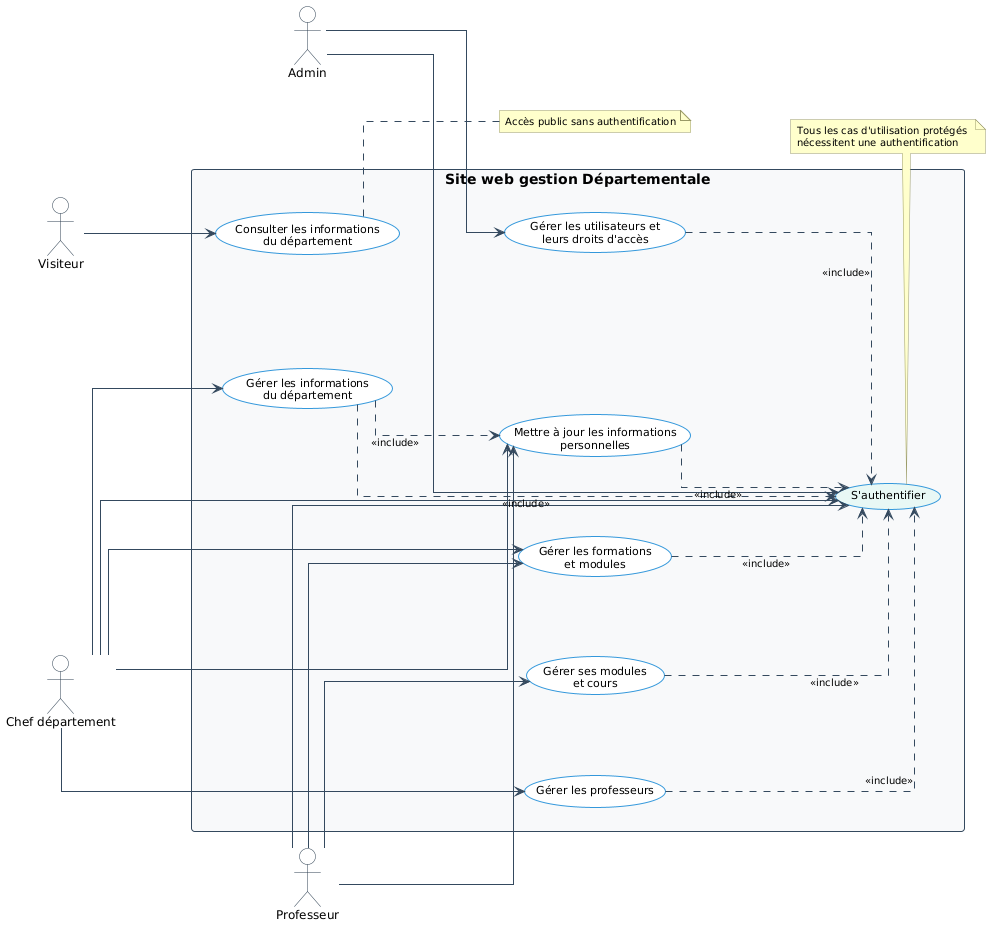
\includegraphics[width=0.8\textwidth]{diagrams/use_case.png} % Assurez-vous que le chemin est correct
    \caption{Diagramme de cas d'utilisation du système}
    \label{fig:use-case-diagram-condensed}
\end{figure}

\subsection{Description des Cas d'Utilisation Principaux}
\begin{itemize}
    \item \textbf{UC1 - Gérer les utilisateurs et droits d'accès (Admin) :} Création, modification, suppression des comptes et gestion des rôles.
    \item \textbf{UC2 - Gérer les informations du département (Chef Dept.) :} Mise à jour des descriptifs, contacts et communication.
    \item \textbf{UC3 - Gérer les professeurs (Chef Dept.) :} Recrutement, affectations, suivi des dossiers.
    \item \textbf{UC4 - Gérer les formations et modules (Chef Dept., Prof.) :} Création/modification des programmes, organisation modulaire.
    \item \textbf{UC5 - Mettre à jour les informations personnelles (Tous authentifiés) :} Modification des données personnelles et professionnelles.
    \item \textbf{UC6 - Gérer ses modules et cours (Prof.) :} Gestion du contenu pédagogique, planification, évaluation.
    \item \textbf{UC7 - Consulter les informations du département (Visiteur, Tous) :} Accès public aux informations générales.
\end{itemize}
\textit{Note : Tous les cas d'utilisation nécessitant une protection incluent implicitement une étape d'authentification.}

\subsection{Diagramme de Séquence}

Le diagramme de séquence global ci-dessous (Figure \ref{fig:sequence-diagram-global}) illustre les interactions typiques entre les principaux composants du Système de Gestion Départementale de l'ENSIAS. Il offre une vue d'ensemble de la manière dont les requêtes des utilisateurs sont traitées à travers les différentes couches de l'application, depuis l'interface utilisateur jusqu'à la base de données.

\begin{figure}[H]
    \centering
    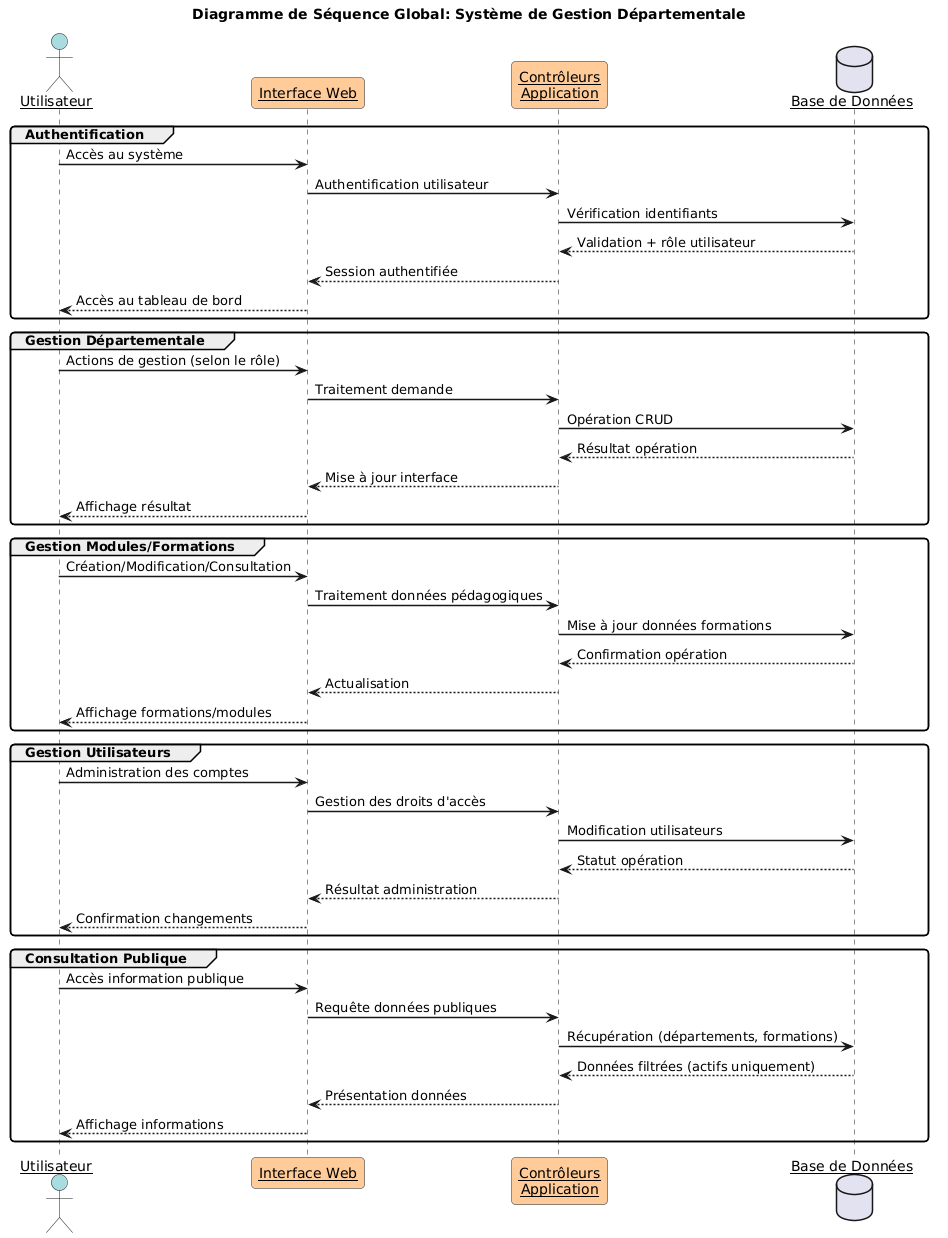
\includegraphics[width=0.9\textwidth]{diagrams/sequence_global.png} % Assurez-vous que le chemin est correct
    \caption{Le Diagramme de Séquence global}
    \label{fig:sequence-diagram-global} % Changé le label pour être unique si besoin
\end{figure}

Les participants clés sont :
\begin{itemize}
    \item \textbf{Utilisateur (Actor)} : Représente toute personne interagissant avec le système.
    \item \textbf{Interface Web (UI)} : La couche de présentation.
    \item \textbf{Contrôleurs Application} : Le cœur logique du système, traitant les requêtes.
    \item \textbf{Base de Données (DB)} : Le système de persistance des données.
\end{itemize}

Le diagramme est structuré en plusieurs groupes représentant des scénarios d'interaction majeurs :
\begin{itemize}
    \item \textbf{Authentification :} Processus de connexion et de validation des identifiants.
    \item \textbf{Gestion Départementale :} Opérations CRUD sur les informations des départements.
    \item \textbf{Gestion Modules/Formations :} Création, modification ou consultation des données pédagogiques.
    \item \textbf{Gestion Utilisateurs :} Administration des comptes et des droits d'accès (principalement par l'Admin).
    \item \textbf{Consultation Publique :} Accès en lecture seule aux informations publiques pour les visiteurs.
\end{itemize}
En résumé, ce diagramme démontre une architecture en couches où l'interface utilisateur est découplée de la logique métier et de la persistance des données, soulignant le flux de contrôle pour les opérations courantes.

\textit{Un diagramme de séquence détaillera les interactions entre objets pour un scénario précis, comme l'inscription d'un nouvel utilisateur ou la gestion d'un module par un professeur.}


\section{Conception de la Base de Données}
La base de données est structurée autour d'un modèle entité-relation.

\subsection{Modèle Entité-Relation}
Le diagramme entité-relation (MER) illustre les entités, leurs attributs et leurs relations.

\begin{figure}[H]
    \centering
    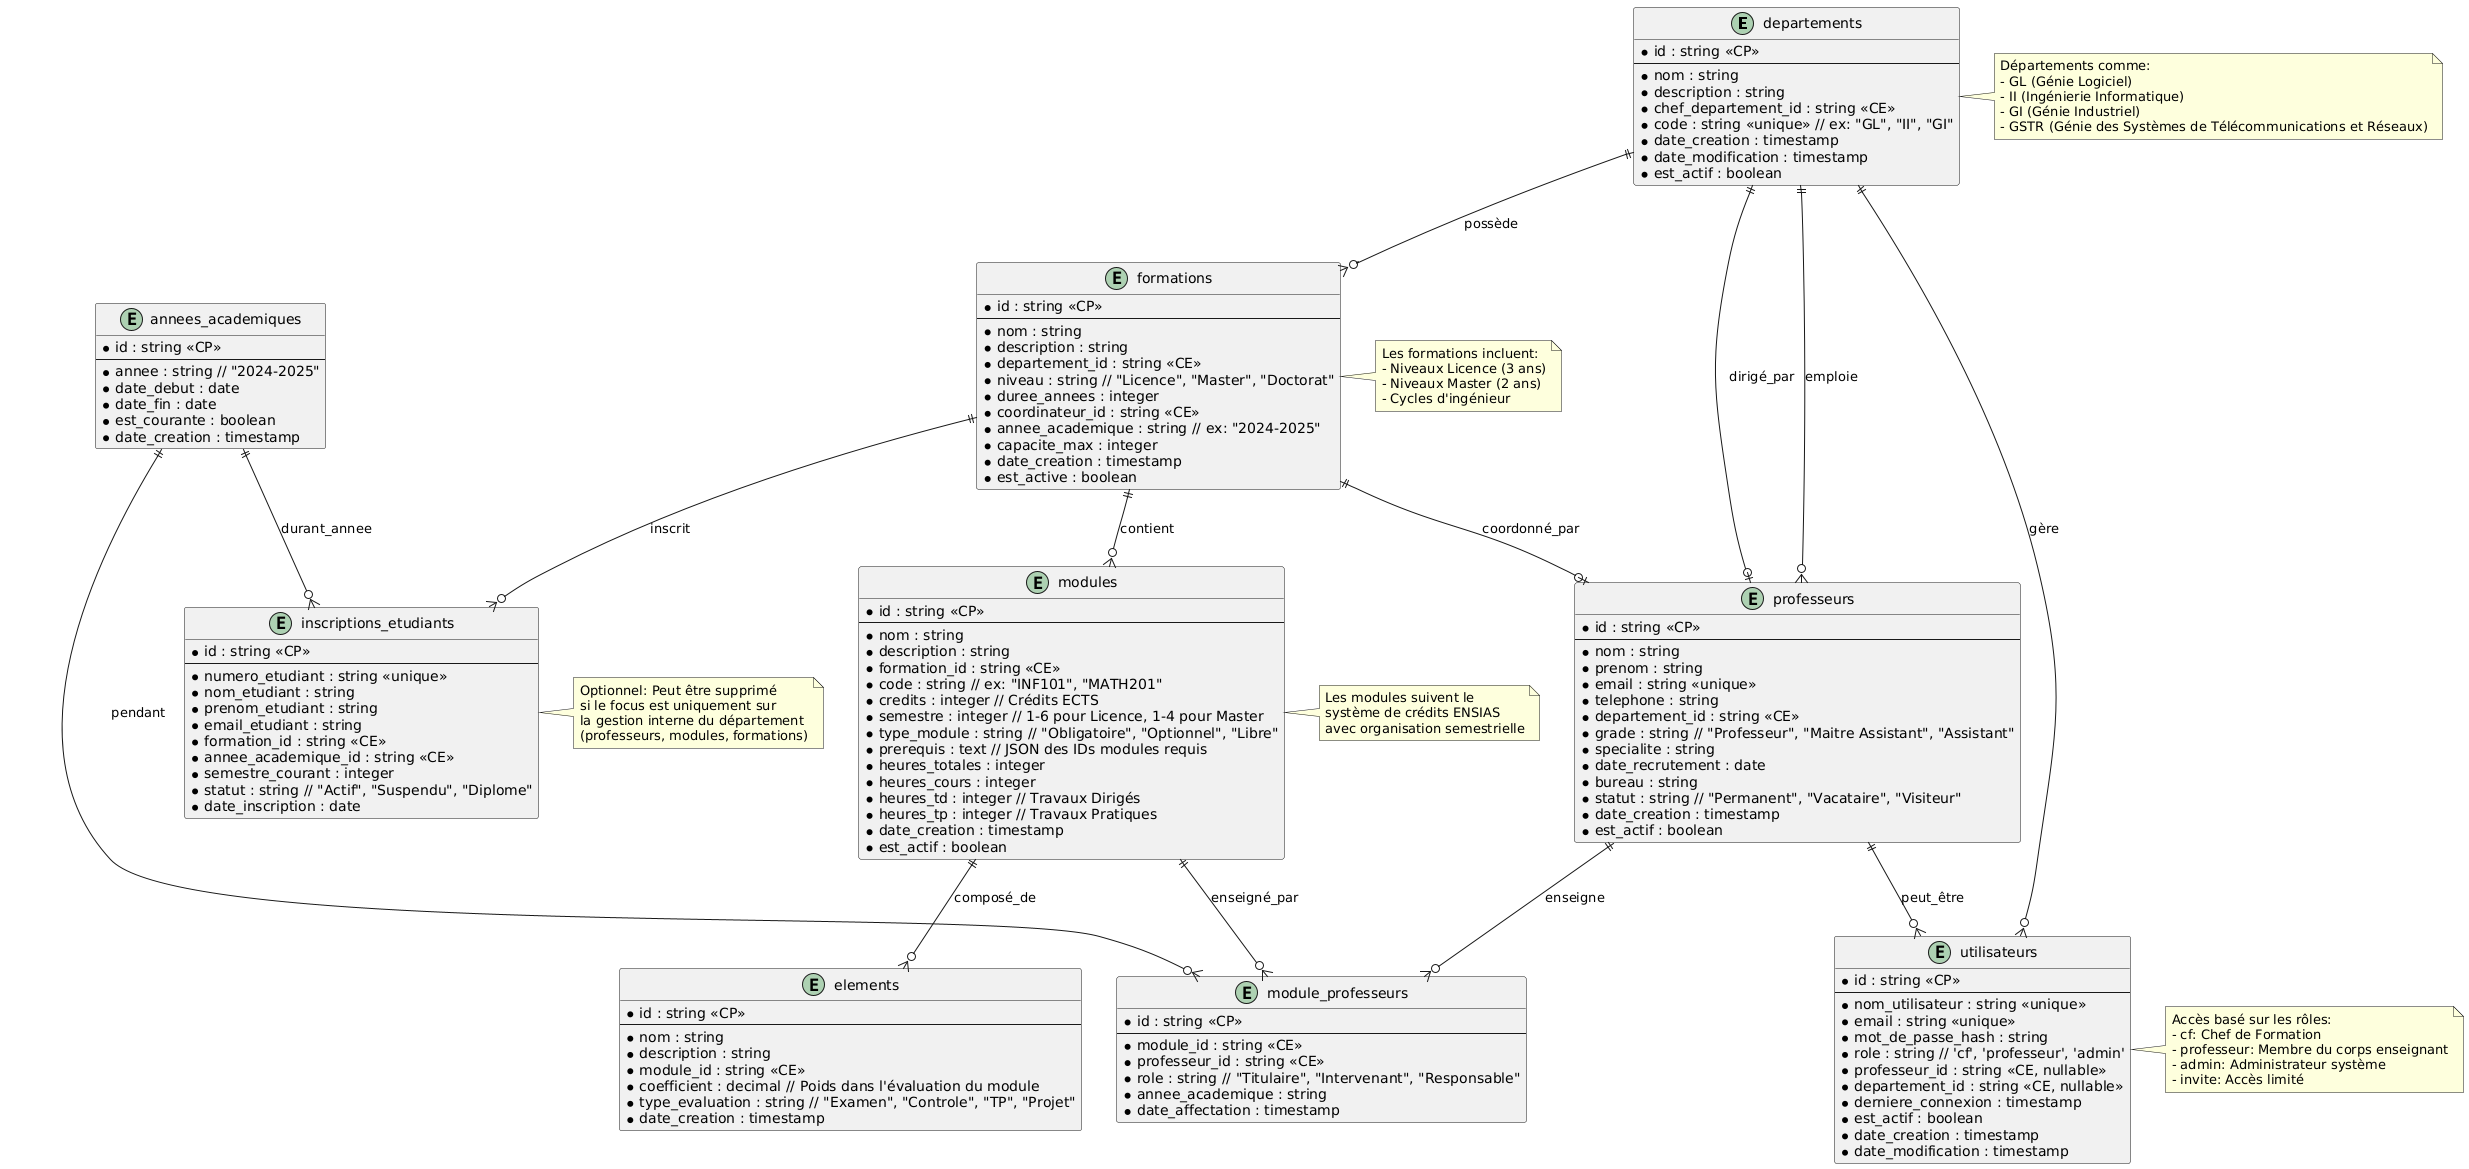
\includegraphics[width=0.9\textwidth]{diagrams/entities.png} % Assurez-vous que le chemin est correct
    \caption{Diagramme entité-relation du système}
    \label{fig:er-diagram-condensed}
\end{figure}

\subsection{Description des Entités Principales}
\begin{itemize}
    \item \textbf{Départements :} Identifiant, nom, code (GL, II, etc.), chef de département (FK).
    \item \textbf{Formations :} Identifiant, nom, type (Licence, Master), capacité, responsable (FK Professeur), département (FK).
    \item \textbf{Modules :} Identifiant, nom, heures (Cours, TD, TP), crédits ECTS, prérequis (JSON), type (obligatoire, optionnel), formation (FK).
    \item \textbf{Éléments de Module :} Identifiant, nom, pondération, type évaluation, module (FK).
    \item \textbf{Professeurs :} Identifiant, nom, prénom, email, grade, spécialité, statut, bureau, département (FK).
    \item \textbf{Utilisateurs :} Identifiant, email, mot de passe haché, rôle (admin, chef, prof), référence optionnelle ProfesseurID.
    \item \textbf{Années Académiques :} Identifiant, libellé (ex: "2023-2024"), date début, date fin, statut (courante, archivée).
    \item \textbf{Module\_Professeurs (Association) :} FK Module, FK Professeur, FK AnnéeAcadémique, rôle (titulaire, intervenant).
\end{itemize}

\subsection{Relations et Cardinalités Clés}
\begin{itemize}
    \item \textbf{Hiérarchiques :} Département (1) -- (*) Formations (1) -- (*) Modules (1) -- (*) Éléments.
    \item \textbf{Affectation :} Professeurs (1) -- (*) Département. Professeurs (*) -- (*) Modules (via Module\_Professeurs).
    \item \textbf{Responsabilité :} Un Professeur dirige un Département. Un Professeur coordonne une Formation.
\end{itemize}

\subsection{Considérations Techniques}
\begin{itemize}
    \item \textbf{Intégrité des données :} Clés primaires et étrangères, contraintes d'unicité (emails, codes) et de domaine.
    \item \textbf{Évolutivité et Maintenance :} Timestamps (création/modification), flags d'activité (soft delete), structure JSON pour flexibilité (prérequis), normalisation.
\end{itemize}

\section{Conclusion (Synthèse de l'Analyse Condensée)}
L'analyse fonctionnelle a défini les acteurs et les fonctionnalités essentielles via les cas d'utilisation. L'analyse non fonctionnelle a souligné les impératifs de sécurité, performance et utilisabilité. La conception de la base de données propose un modèle relationnel structuré pour supporter ces fonctionnalités, avec une attention portée à l'intégrité et à l'évolutivité.
Les défis principaux résident dans la gestion des aspects temporels (années académiques), l'optimisation des performances et la création d'interfaces utilisateurs ergonomiques.
